\section{Memory management}

My goal for this part was to store the data read from buttons driver in a single memory location and then read it plotting tha value by means of the array of leds on the Altera board. First of all I had to implement the memory controller to run access protocols, but in any case I no reached to synchronize correctly the manager and the memory. In the end, my memory controller just emulates the access protocols, satisfying the waveform shapes for each clock cycles; however any consideration about access time or similar have been discharged.
\newline
Two words about the target memory. It's a 256 Mbits SDRAM provided by ISSI. It's fully synchronous, offers the possibility to do burst transfers, does auto-refreshing, allows programmable CAS latency and so on.
\newline
\newline
As first, I needed to know how FPGA is interfaced with SDRAM.
\begin{figure}[H]
\centering
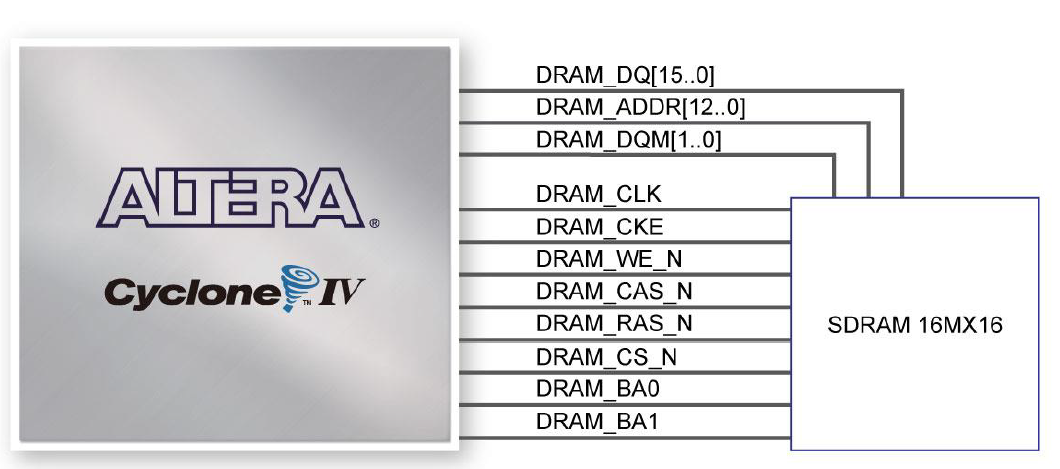
\includegraphics[scale=.7]{Immagini/25}
\label{25}
\caption{Connections between FPGA chip and SDRAM}
\end{figure}

There are 13 bits of address $Ax$ and 16 bits input/output for data. The SDRAM is composed of 4 banks 8192 size each; to select one of them 2 input bits called Bank Select Address are used. Then the clock and clock enable are inputs as well. Moreover, there are the chip select, the write enable, the row address strobe and the column address strobe, all of them active low. This SDRAM offers possibility to mask the output, driving the 2 Data Masked bits, for the high and low parts respectively.
\newline
\newline
My module is a classic finite state machine, where each step is generated on the rising edge of the clock. The FSM is composed of 20 states. Looking at the datasheet, the state diagram is more complex so I decided to build it implementing the basic operations: the initialization, the programming,  the request of a read the the request of a write. In between, memory expects to be precharged and refreshed. What I'm going to show in this section is the comparison between waveforms I'm able to generate and what is shown in the datasheet.
\newpage


\begin{lstlisting}[caption=VHDL entity of memory manager, language=VHDL]
entity MemoryInterface is
	port(
		MI_buttons : in std_logic_vector(7 downto 0);
		MI_clk	 : in std_logic;
		MI_reset : in std_logic;
		MI_enable : in std_logic;
		MI_RW : in std_logic; -- external event, no event reading, event writing
		MI_action : in std_logic; -- active low
		MI_address : in std_logic_vector(14 downto 0);
		
--		real interface
		
		MI_address_9_0 : out std_logic_vector(9 downto 0);
		MI_address_10 : out std_logic;
		MI_address_12_11: out std_logic_vector(12 downto 11);
		MI_bank : out std_logic_vector(1 downto 0);
		MI_data : inout std_logic_vector(15 downto 0);
		MI_CAS : out std_logic; -- active low
		MI_RAS : out std_logic; -- active low
		MI_CS : out std_logic; -- active low
		MI_write_enable : out std_logic; -- active low
		MI_clk_enable : out std_logic; -- active high
		MI_memory_clk : out std_logic;
		MI_DQML : out std_logic;
		MI_DQMH : out std_logic
	);
end MemoryInterface;
\end{lstlisting}

\begin{figure}[H]
\centering
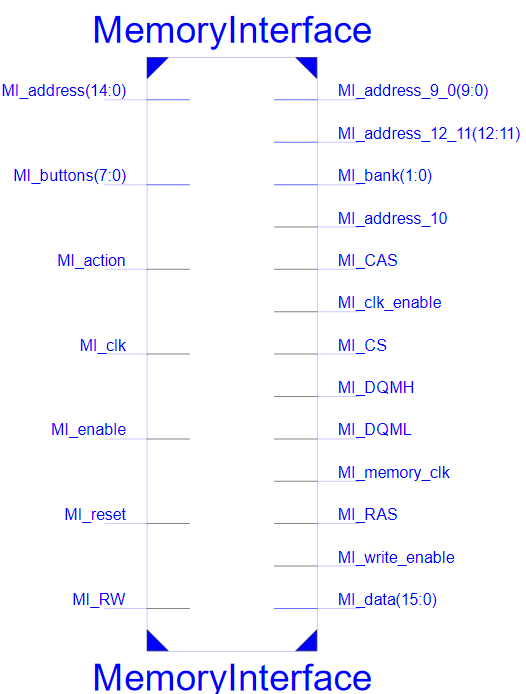
\includegraphics[scale=.6]{Immagini/27}
\label{27}
\caption{Memory interface pinout}
\end{figure}

\begin{figure}[H]
\centering
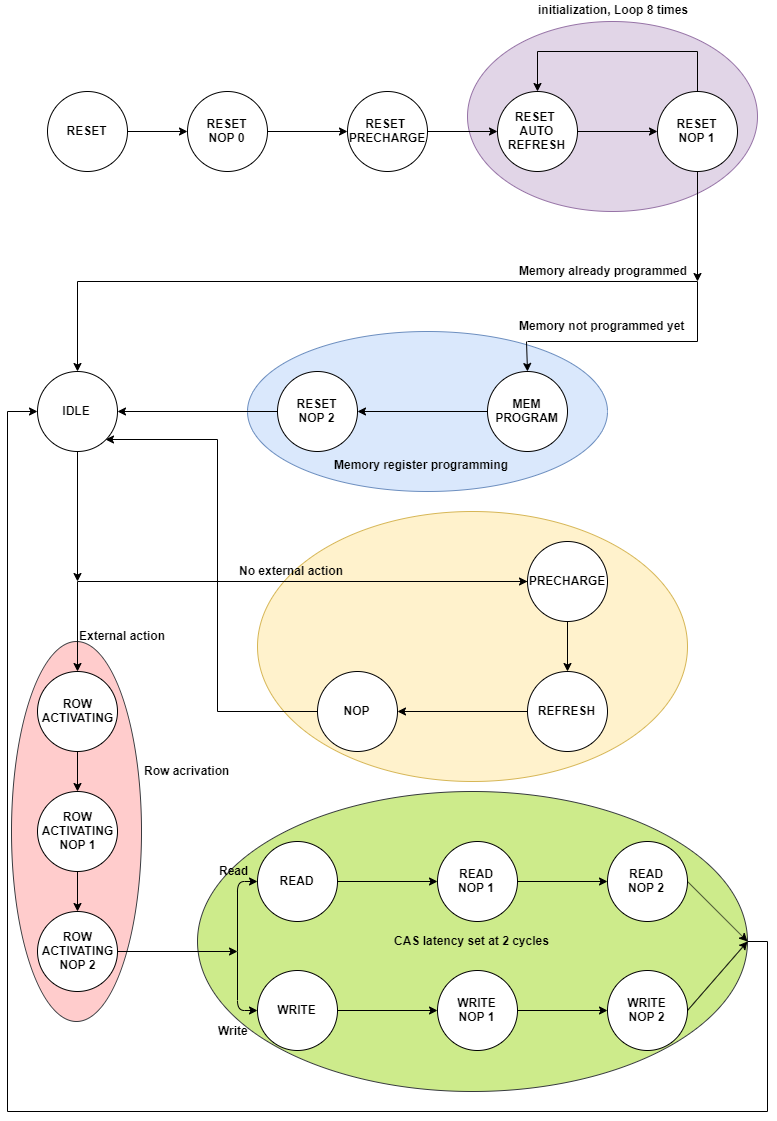
\includegraphics[scale=.6]{Immagini/26}
\label{26}
\caption{Memory controller state diagram}
\end{figure}

\begin{figure}[H]
\centering
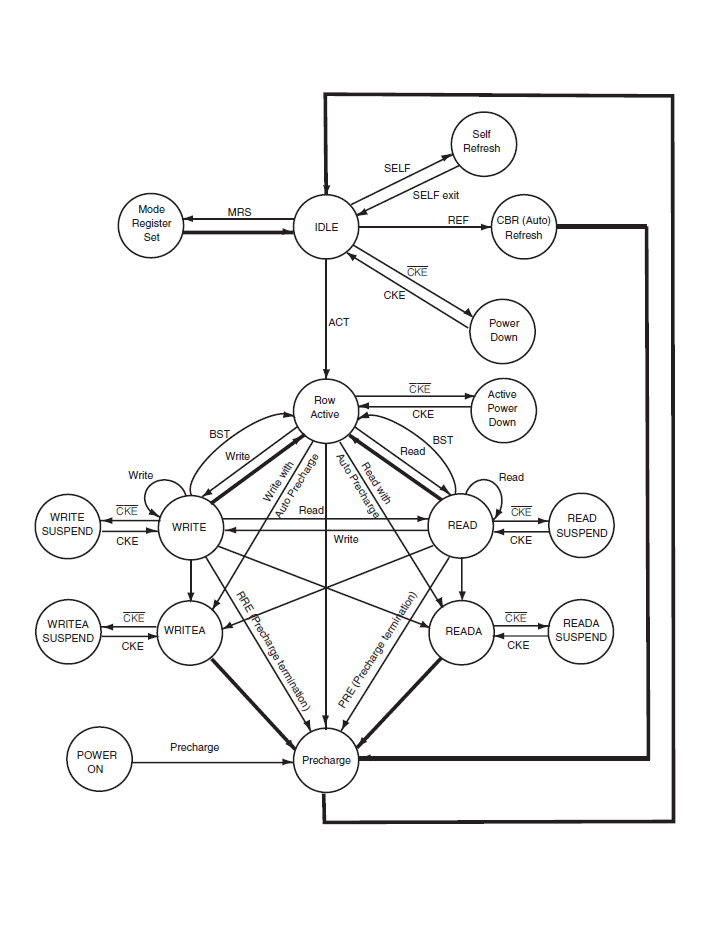
\includegraphics[scale=1.1]{Immagini/34}
\label{26}
\caption{Memory state diagram from datasheet}
\end{figure}

When reset pin has activated, the SDRAM is once precharged, then for 8 times alternates a cycle of refreshing and one cycle of NOP. The bit 10 of the address, provides memory information about refreshing. If it's '1' all banks are refreshed, otherwise only the one is indicated by MI\_bank bits. After initialization, the manager should be program the control register of the memory, which provides some information such as: burst length (1), burst type (sequential), CAS latency (2) and write burst mode (single location access). The state memory load register follows the end of initialization loop.

\begin{figure}[H]
\centering
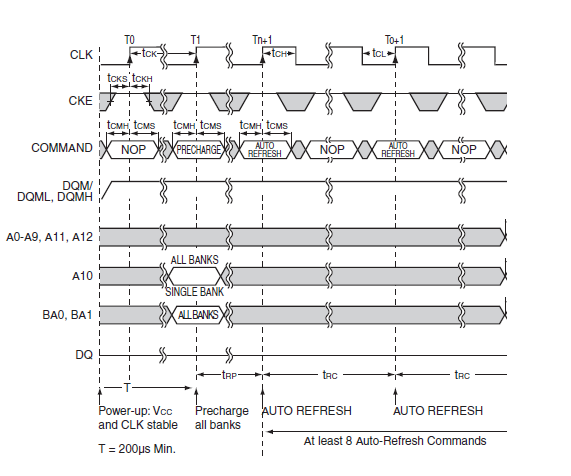
\includegraphics{Immagini/29}
\label{29}
\caption{Initialization: datasheet}
\end{figure}

\begin{figure}[H]
\centering
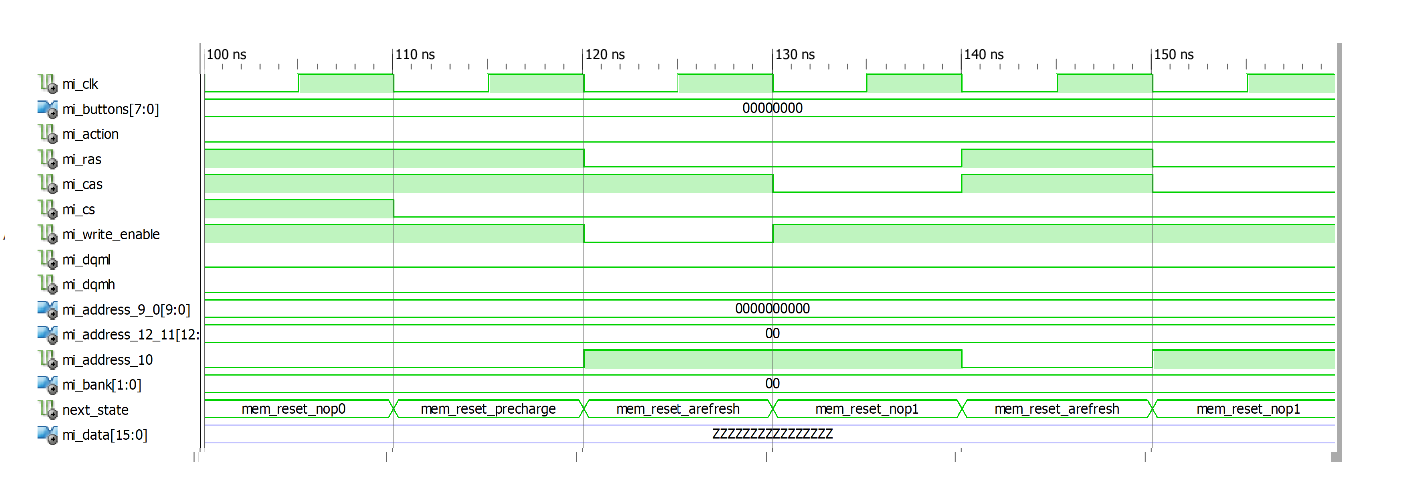
\includegraphics[scale=.5]{Immagini/28}
\label{28}
\caption{Initialization: simulation}
\end{figure}
\newpage
From the idle state, the controller detects that an action has been driven from outside. From idle the state diagram moves toward the activation on the target row, which is passed on address pins and recognized by activating the row address strobe. After two cycles, memory controller sends the data and the column address, activating the CAS in the meantime. Since CAS latency has been set to 2 cycles, memory requires two NOP cycles to accomplish the operation. Small note for the reader: both read and write can be performed with or without auto-precharging, depending on the logic value on the 10th bit of address. Due to the fact that, in datasheet, the time diagrams of write both with auto precharge and without are totally equal, while read diagrams differ from the explicit presence of that (how we will see next), I guess that write with auto precharging diagram is wrong. Precharging command should not be sent from memory controller.

\begin{figure}[H]
\centering
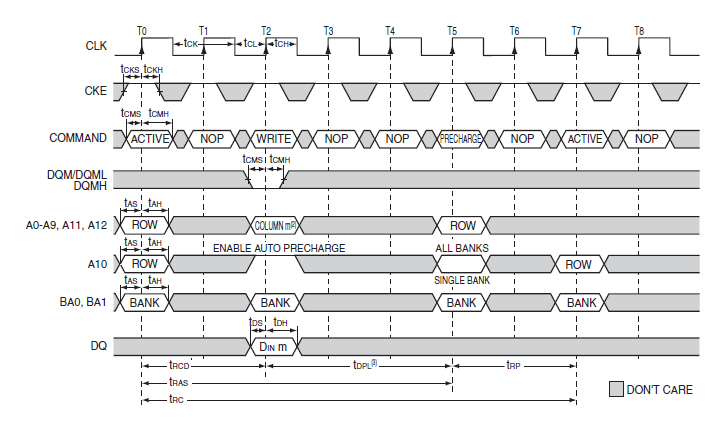
\includegraphics[scale=.9]{Immagini/31}
\label{31}
\caption{Write: datasheet}
\end{figure}

\begin{figure}[H]
\centering
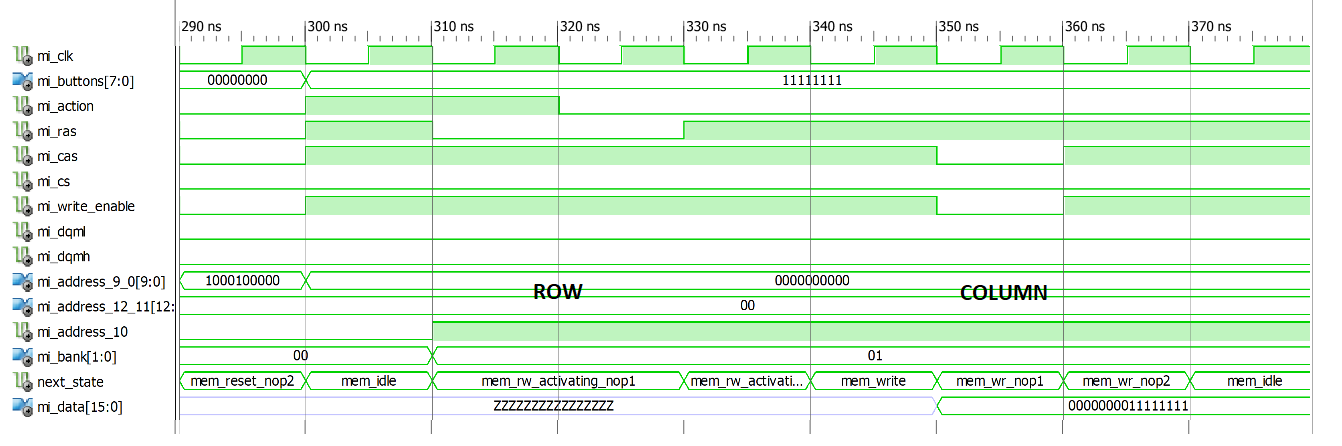
\includegraphics[scale=.5]{Immagini/30}
\label{30}
\caption{Write: simulation}
\end{figure}

\newpage

As you can see from the datasheet diagram, when the operation has been set with autoprecharging, that command is not sent but automatically performed by memory internally. 

\begin{figure}[H]
\centering
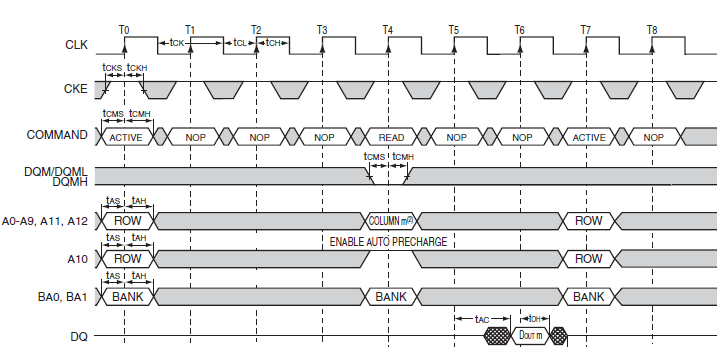
\includegraphics[scale=.9]{Immagini/33}
\label{33}
\caption{Read: datasheet}
\end{figure}

\begin{figure}[H]
\centering
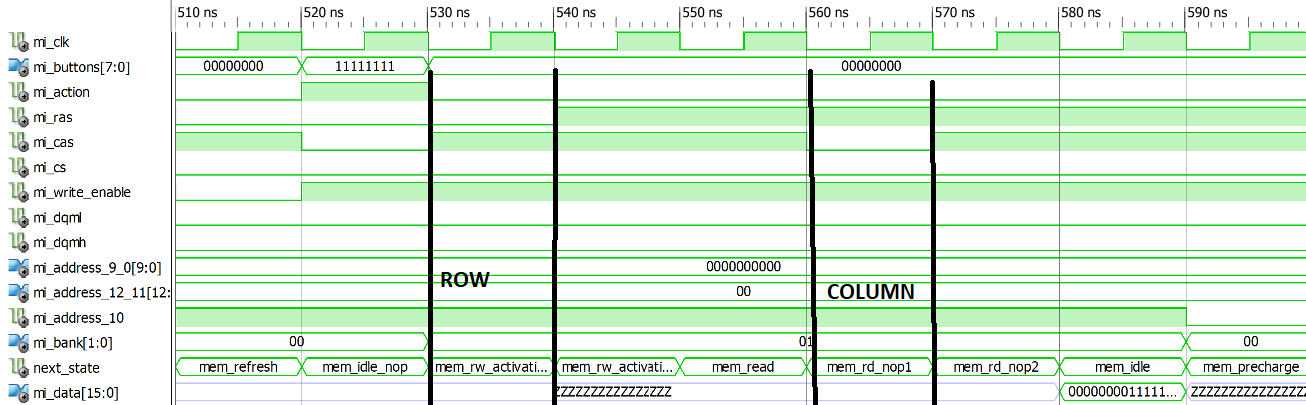
\includegraphics[scale=.5]{Immagini/32}
\label{32}
\caption{Read: simulation}
\end{figure}

\begin{figure}[H]
\centering
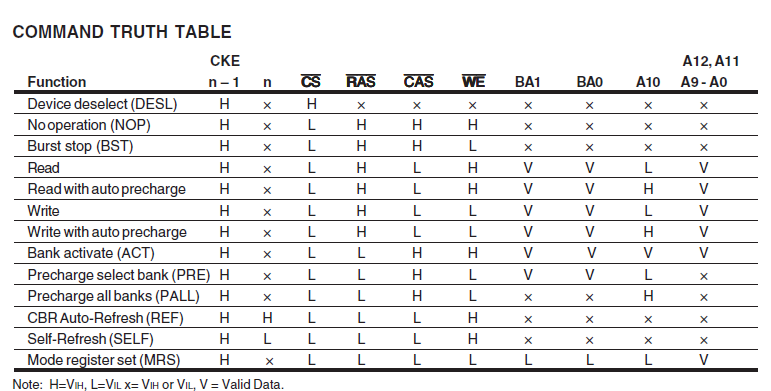
\includegraphics[scale=.8]{Immagini/35}
\label{35}
\caption{Main commands format}
\end{figure}